\documentclass[11pt, oneside]{article} 
\usepackage{geometry}
\geometry{letterpaper} 
\usepackage{graphicx}
	
\usepackage{amssymb}
\usepackage{amsmath}
\usepackage{parskip}
\usepackage{color}
\usepackage{hyperref}

\graphicspath{{/Users/telliott/Dropbox/Github-Math/quickgeo/figures/}{/Users/telliott/Dropbox/Github-Math/figures/}}
% \begin{center} \includegraphics [scale=0.4] {gauss3.png} \end{center}

\title{Trigonometry}
\date{}

\begin{document}
\maketitle
\Large

%[my-super-duper-separator]

\subsection*{definitions}

The sine and cosine are really more a convenience than a necessity in basic geometry, they allow us to use one symbol for the ratio of two sides.  It is only when we come to consider them as functions, and see their utility for modeling periodic phenomena, that they because extremely important.  

Here we just scratch the surface.

I will define them in a slightly different way than usual, and then show the connection:
\begin{center} 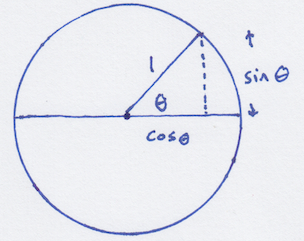
\includegraphics [scale=0.6] {L1b.png} \end{center}

If you draw a right triangle in a unit circle with angle $\theta$ as the central angle, then the sides of the triangle are $\cos \theta$ and $\sin \theta$.

If the triangle and circle are resized so that the length of the radius is $h$, then the $x$ part of the triangle (the side adjacent to the angle) becomes $h \cos \theta$, and the $y$ part of the triangle (the side opposite the angle) becomes $h \sin \theta$.
\[ y = h \sin \theta \]
\[ x = h \cos \theta \]
\begin{center} 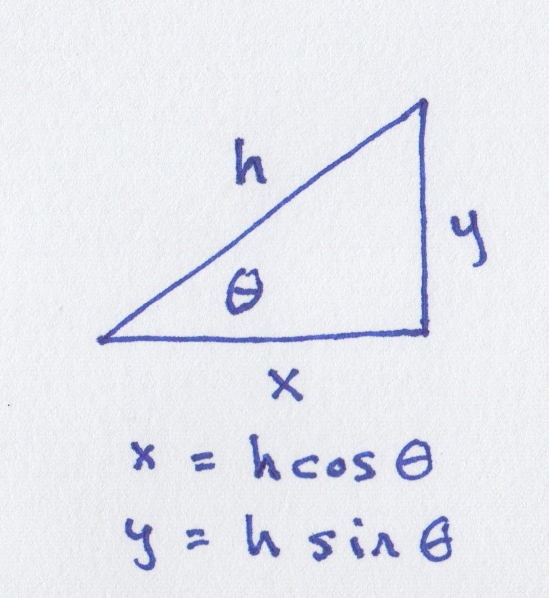
\includegraphics [scale=1.0] {L1c.png} \end{center}

Rearranging slightly:
\[ \frac{y}{h} = \sin \theta \]
\[ \frac{x}{h} = \cos \theta \]

This is the normal presentation.  People recite sine is \emph{opposite over hypotenuse} and cosine is \emph{adjacent over hypotenuse}, but there seems to be endless confusion over this, so I am starting here from a different, but equivalent, viewpoint.

The Pythagorean theorem can be restated as
\[ \sin^2 \theta + \cos^2 \theta = 1 \]
\begin{center} 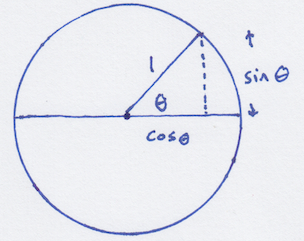
\includegraphics [scale=0.6] {L1b.png} \end{center}

It is an unusual but standard notation that $\sin^2 x$ is written for $(\sin x)^2$ and the same for cosine.

\subsection*{laws of sines and cosines}

Next we look at 2 powerful relationships that are easily derived from these definitions.

\begin{center} 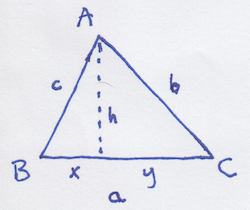
\includegraphics [scale=0.6] {L2.png} \end{center}

The first law is the law of sines.
\[ h = c \sin B, \ \ \ \ \ \ h = b \sin C \]
\[ \frac{\sin B}{b} = \frac{\sin C}{c} \]

By symmetry
\[ \frac{\sin A}{a} = \frac{\sin B}{b} = \frac{\sin C}{c} \]

The second law is the law of cosines.  Again we use $h$ (or rather, $h^2$) to connect two equal expressions.  We also have $y = a - x$.

\[ c^2 - x^2 = h^2 = b^2 - (a - x)^2 \]
\[ a^2 + c^2 = b^2 + 2ax \]
 
 \begin{center} 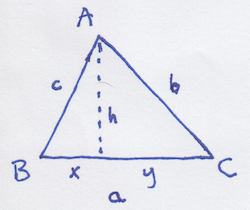
\includegraphics [scale=0.6] {L2.png} \end{center}

But $x = c \cos B$ so
\[ b^2 = a^2 + c^2 - 2ac \cos B \]

Generally, for any angle we can rewrite the formula in terms of the square of the opposite side.

\subsection*{special values}

Since $\theta$ is duplicated in a 45-45-90 right triangle, we have
\[ \sin 45 = \cos 45 = \frac{1}{\sqrt{2}} \]

Cutting an equilateral triangle in half, if the original side is $2$, we obtain
\[ \sin 30 = \frac{1}{2} \]
\[ \cos 30 = \frac{1}{\sqrt{3}} \]

\begin{center} 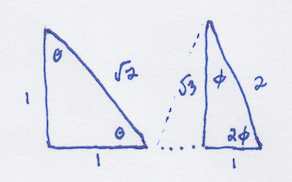
\includegraphics [scale=0.6] {L3.png} \end{center}

The complementary angle switches adjacent and opposite sides (see above), so
\[ \sin 30 = \cos 60 \]
\[ \cos 30 = \sin 60 \]

Another useful tidbit is that if $\theta'$ is supplementary to $\theta$ ($\theta + \theta' = 180$), then $\sin \theta = \sin \theta'$.

\subsection*{ratios of sides}

In the chapter on area, we showed a different proof of the following theorem.  Here we rely on the law of sines.

The angle on the left is bisected.  I claim that $a$ is to $x$ as $b$ is to $y$.
\begin{center} 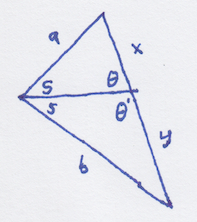
\includegraphics [scale=0.7] {L8.png} \end{center}

We have that 
\[ \frac{x}{\sin s} = \frac{a}{\sin \theta}, \ \ \ \ \ \ \frac{y}{\sin s} = \frac{b}{\sin \theta'} \]

But $\theta$ and $\theta'$ are supplementary so their sines are equal.  Therefore
\[ \frac{x}{a} = \frac{\sin s}{\sin \theta} = \frac{y}{b} \]

$\square$

\subsection*{double scoop problem}

We have two lines tangent to two circles that just touch each other, the smaller one of radius $r$, and the larger of radius $R$.

\begin{center} \includegraphics [scale=0.5] {double_scoop1.png} \end{center}

There is a simple expression for the sine and cosine of $\theta$, the angle between the base and the line through both centers.  The distance between the centers of the two circles is $r + R$.  Draw a horizontal line through the center of the smaller circle.

\begin{center} \includegraphics [scale=0.5] {double_scoop2.png} \end{center}

We have constructed a right triangle, which is similar to the original one.  It includes the angle $\theta$ and the hypotenuse is the distance between the two centers, $R + r$.  The opposite side has length $R - r$ and so
\[ \sin \theta = \frac{R - r}{R + r} \]

The adjacent side (the line segment colored black) has its squared length equal to 
\[ (R + r)^2 - (R - r)^2 = 4Rr \]
thus
\[ \cos \theta = \frac{2 \sqrt{Rr}}{R + r} \]

You can confirm that the identity $\sin^2 \theta + \cos^2 \theta = 1$ works here.

\subsection*{area}

The radius of the circumcircle of the triangle can be expressed in terms of the side lengths.

Draw $\angle D$ on a diameter.  By equal arcs subtended $\angle D = \angle C$.  And by Thales' circle theorem, the $\angle ABD$ is a right angle.  
\begin{center} 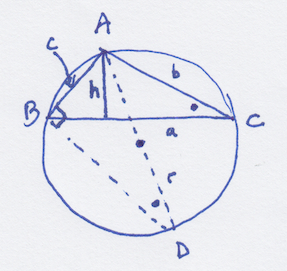
\includegraphics [scale=0.6] {L4.png} \end{center}

As a result $\triangle ABD \sim$ the right triangle formed with one vertex at $C$ and third at $A$.  $h$ is the side opposite $\angle C$.

We have that the ratios of the short side to the hypotenuse are:
\[ \frac{h}{b} = \frac{c}{2r} \]
\[ r = \frac{bc}{2h} \]

We also have that twice the area of $\triangle ABC$, written $2(ABC)$ is equal to $ha$.  Substituting for $h$:
\[ r = \frac{abc}{4(ABC)} \]

\subsection*{another method}

If we go back to the first example of the inscribed angle theorem, we have that the central angle is twice the peripheral angle subtending the same arc.
\begin{center} 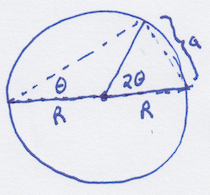
\includegraphics [scale=0.6] {L5.png} \end{center}

\[ \frac{a}{2R} = \sin \theta \]

But $\theta$ can move anywhere on the circle
\begin{center} 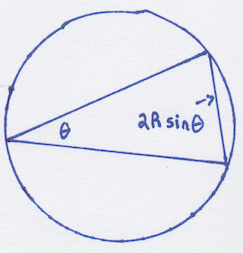
\includegraphics [scale=0.6] {L6.png} \end{center}
\[ a = 2R \sin \theta \]

As before, except we switched $r$ for $R$
\begin{center} 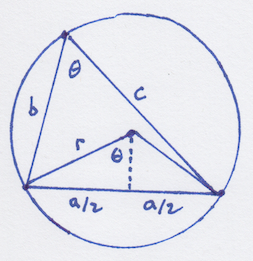
\includegraphics [scale=0.6] {L7.png} \end{center}

The altitude to side $c$ is $b \sin \theta$, so the area of the triangle (symbolized by $\triangle$) is
\[ \triangle = \frac{bc \sin \theta}{2} \]

We substitute for $\sin \theta = a/2r$:
\[ \triangle = \frac{abc}{4r} \]

which is rearranged to
\[ r = \frac{abc}{4 \triangle} \]


\end{document}